% ---------------------------------------------------------------------------
% Workflow of the performance-portability study.
%
% Renders the four stages of the pipeline (provision, configure & build,
% run & verify, analyze) together with the repository that provides each of
% them. Build the figure with:
%
%   pdflatex -output-directory=docs docs/workflow.tex
%   magick -density 200 docs/workflow.pdf -background white \
%       -alpha remove -alpha off docs/workflow.png
%
% ---------------------------------------------------------------------------
\documentclass[border=4pt,tikz]{standalone}

\usepackage[T1]{fontenc}
\usepackage{lmodern}
\usepackage{amsmath}
\usetikzlibrary{arrows.meta,positioning,shapes.arrows,calc}

% Palette shared with the methodology figure of the paper.
\definecolor{ppbBlue}{RGB}{0,82,147}
\definecolor{ppbHeader}{RGB}{6,88,145}
\definecolor{ppbBand}{RGB}{100,163,202}
\definecolor{ppbLight}{RGB}{229,239,248}
\definecolor{ppbArrowTop}{RGB}{225,234,250}
\definecolor{ppbArrowBottom}{RGB}{128,163,221}
% One accent colour per repository so that every stage can be attributed.
\definecolor{repoBoot}{RGB}{247,197,142}
\definecolor{repoBootLight}{RGB}{253,231,204}
\definecolor{repoBench}{RGB}{154,166,236}
\definecolor{repoBenchLight}{RGB}{219,223,250}
\definecolor{repoPpbcc}{RGB}{165,226,174}
\definecolor{repoPpbccLight}{RGB}{223,246,227}

\begin{document}
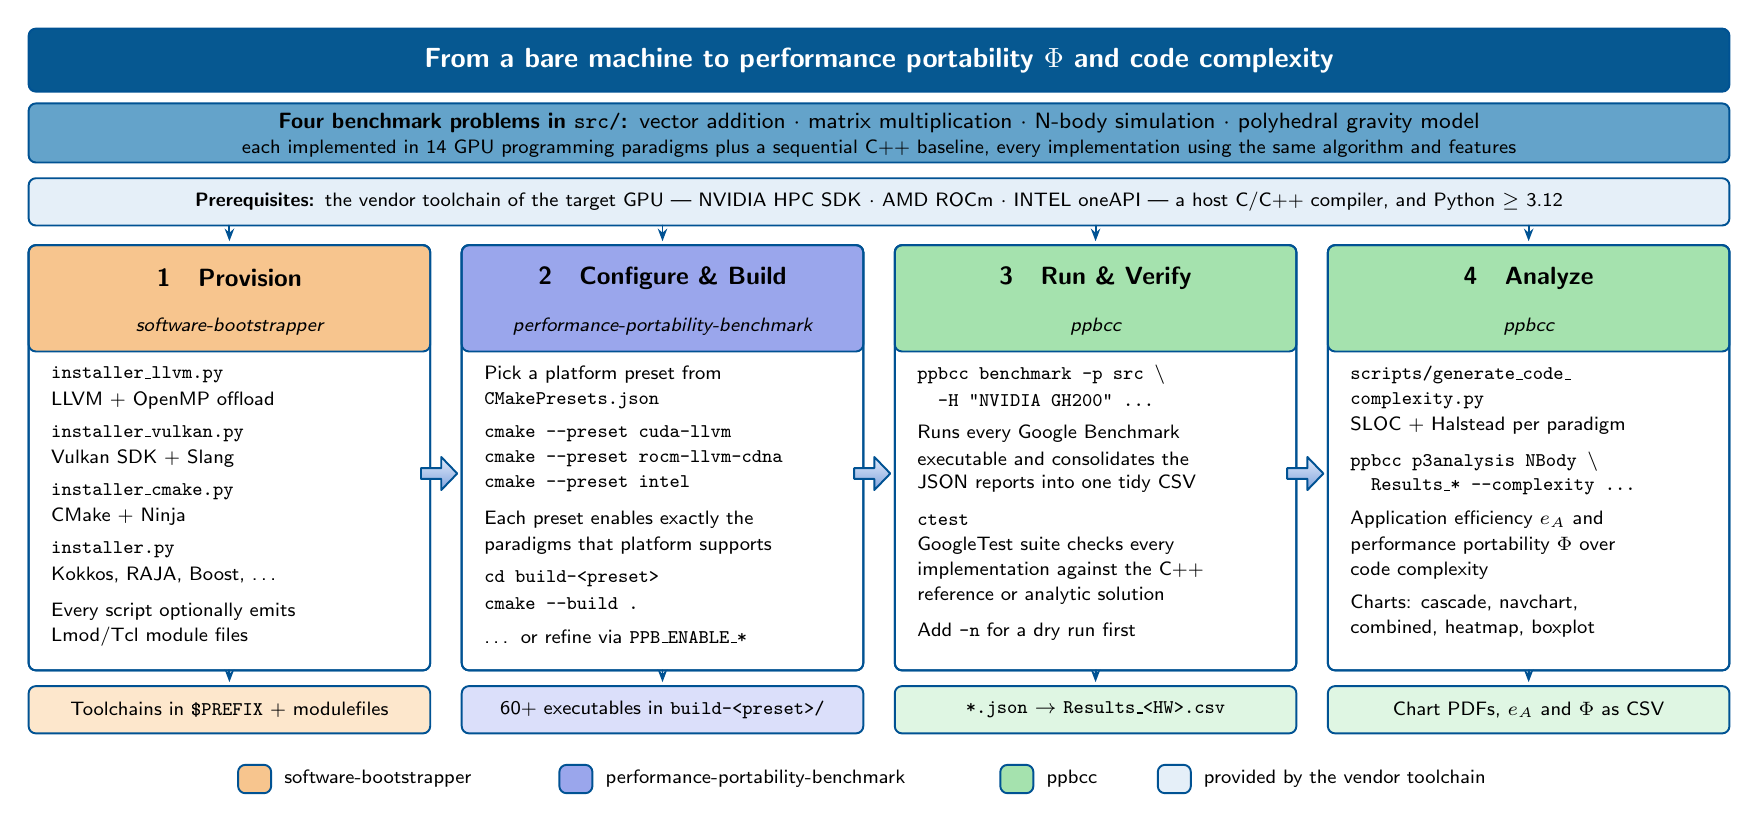
\begin{tikzpicture}[
    x=1cm,
    y=1cm,
    line cap=round,
    line join=round,
    card/.style={rounded corners=2.6pt, line width=0.7pt, draw=ppbBlue},
    stage title/.style={font=\sffamily\bfseries\small, align=center, inner sep=0pt},
    repo tag/.style={font=\sffamily\scriptsize\itshape, align=center, inner sep=0pt},
    desc/.style={font=\sffamily\scriptsize, align=left, inner sep=0pt, anchor=west},
    mono/.style={font=\ttfamily\scriptsize, align=left, inner sep=0pt, anchor=west},
    band text/.style={font=\sffamily\footnotesize, align=center, inner sep=0pt},
    chip text/.style={font=\sffamily\scriptsize, align=center, inner sep=0pt},
    legend text/.style={font=\sffamily\scriptsize, align=left, inner sep=0pt, anchor=west},
    flow arrow/.style={
        single arrow,
        inner sep=0pt,
        inner ysep=1.0pt,
        single arrow head extend=0.10cm,
        single arrow tip angle=92,
        draw=ppbBlue,
        line width=0.7pt,
        top color=ppbArrowTop,
        bottom color=ppbArrowBottom,
        minimum width=0.42cm,
        minimum height=0.46cm,
        anchor=tip
    }
]

    % ----------------------------------------------------------------------
    % Layout (units: cm, origin bottom left), total 21.60 x 9.85
    %   9.05--9.85  overall title band
    %   8.15--8.90  what is benchmarked
    %   7.35--7.95  prerequisites
    %   5.75--7.10  four stage cards, header strip
    %   1.70--5.75  four stage cards, body
    %   0.90--1.50  one output chip below every card
    %   0.14--0.50  legend
    % Stage cards are 5.10 wide, separated by 0.40 gaps that hold the arrows.
    % ----------------------------------------------------------------------

    \def\cardw{5.10}
    \def\cardtop{7.10}
    \def\cardbot{1.70}
    \def\headerbot{5.75}

    % ------------------------------------------------------------------
    % Title and context bands
    % ------------------------------------------------------------------
    \fill[ppbHeader, card] (0,9.05) rectangle (21.60,9.85);
    \node[stage title, text=white, font=\sffamily\bfseries\normalsize] at (10.80,9.45)
        {From a bare machine to performance portability \(\Phi\) and code complexity};

    \fill[ppbBand, card] (0,8.15) rectangle (21.60,8.90);
    \node[band text, text width=21.00cm] at (10.80,8.65)
        {\textbf{Four benchmark problems in \texttt{src/}:}
         vector addition \(\cdot\) matrix multiplication \(\cdot\)
         N-body simulation \(\cdot\) polyhedral gravity model};
    \node[band text, text width=21.00cm, font=\sffamily\scriptsize] at (10.80,8.32)
        {each implemented in 14 GPU programming paradigms plus a sequential C++ baseline,
         every implementation using the same algorithm and features};

    \fill[ppbLight, card] (0,7.35) rectangle (21.60,7.95);
    \node[band text, text width=21.00cm, font=\sffamily\scriptsize] at (10.80,7.65)
        {\textbf{Prerequisites:} the vendor toolchain of the target GPU ---
         NVIDIA HPC SDK \(\cdot\) AMD ROCm \(\cdot\) INTEL oneAPI ---
         a host C/C++ compiler, and Python \(\geq\) 3.12};

    % ------------------------------------------------------------------
    % Stage 1 -- Provision
    % ------------------------------------------------------------------
    \begin{scope}[shift={(0,0)}]
        \fill[white, card] (0,\cardbot) rectangle (\cardw,\cardtop);
        \fill[repoBoot, card] (0,\headerbot) rectangle (\cardw,\cardtop);
        \draw[card] (0,\cardbot) rectangle (\cardw,\cardtop);
        \node[stage title] at (2.55,6.68) {1\quad Provision};
        \node[repo tag] at (2.55,6.06) {software-bootstrapper};

        \node[mono] at (0.28,5.45) {installer\_llvm.py};
        \node[desc] at (0.28,5.13) {LLVM + OpenMP offload};
        \node[mono] at (0.28,4.71) {installer\_vulkan.py};
        \node[desc] at (0.28,4.39) {Vulkan SDK + Slang};
        \node[mono] at (0.28,3.97) {installer\_cmake.py};
        \node[desc] at (0.28,3.65) {CMake + Ninja};
        \node[mono] at (0.28,3.23) {installer.py};
        \node[desc] at (0.28,2.91) {Kokkos, RAJA, Boost, \dots};
        \node[desc] at (0.28,2.45) {Every script optionally emits};
        \node[desc] at (0.28,2.13) {Lmod/Tcl module files};
    \end{scope}

    % ------------------------------------------------------------------
    % Stage 2 -- Configure and build
    % ------------------------------------------------------------------
    \begin{scope}[shift={(5.50,0)}]
        \fill[white, card] (0,\cardbot) rectangle (\cardw,\cardtop);
        \fill[repoBench, card] (0,\headerbot) rectangle (\cardw,\cardtop);
        \draw[card] (0,\cardbot) rectangle (\cardw,\cardtop);
        \node[stage title] at (2.55,6.68) {2\quad Configure \& Build};
        \node[repo tag] at (2.55,6.06) {performance-portability-benchmark};

        \node[desc] at (0.28,5.45) {Pick a platform preset from};
        \node[mono] at (0.28,5.13) {CMakePresets.json};
        \node[mono] at (0.28,4.71) {cmake -{}-preset cuda-llvm};
        \node[mono] at (0.28,4.39) {cmake -{}-preset rocm-llvm-cdna};
        \node[mono] at (0.28,4.07) {cmake -{}-preset intel};
        \node[desc] at (0.28,3.61) {Each preset enables exactly the};
        \node[desc] at (0.28,3.29) {paradigms that platform supports};
        \node[mono] at (0.28,2.87) {cd build-<preset>};
        \node[mono] at (0.28,2.55) {cmake -{}-build .};
        \node[desc] at (0.28,2.13) {\dots{} or refine via \texttt{PPB\_ENABLE\_*}};
    \end{scope}

    % ------------------------------------------------------------------
    % Stage 3 -- Run and verify
    % ------------------------------------------------------------------
    \begin{scope}[shift={(11.00,0)}]
        \fill[white, card] (0,\cardbot) rectangle (\cardw,\cardtop);
        \fill[repoPpbcc, card] (0,\headerbot) rectangle (\cardw,\cardtop);
        \draw[card] (0,\cardbot) rectangle (\cardw,\cardtop);
        \node[stage title] at (2.55,6.68) {3\quad Run \& Verify};
        \node[repo tag] at (2.55,6.06) {ppbcc};

        \node[mono] at (0.28,5.45) {ppbcc benchmark -p src \(\backslash\)};
        \node[mono] at (0.28,5.13) {~~-H "NVIDIA GH200" \dots};
        \node[desc] at (0.28,4.71) {Runs every Google Benchmark};
        \node[desc] at (0.28,4.39) {executable and consolidates the};
        \node[desc] at (0.28,4.07) {JSON reports into one tidy CSV};
        \node[mono] at (0.28,3.61) {ctest};
        \node[desc] at (0.28,3.29) {GoogleTest suite checks every};
        \node[desc] at (0.28,2.97) {implementation against the C++};
        \node[desc] at (0.28,2.65) {reference or analytic solution};
        \node[desc] at (0.28,2.19) {Add \texttt{-n} for a dry run first};
    \end{scope}

    % ------------------------------------------------------------------
    % Stage 4 -- Analyze
    % ------------------------------------------------------------------
    \begin{scope}[shift={(16.50,0)}]
        \fill[white, card] (0,\cardbot) rectangle (\cardw,\cardtop);
        \fill[repoPpbcc, card] (0,\headerbot) rectangle (\cardw,\cardtop);
        \draw[card] (0,\cardbot) rectangle (\cardw,\cardtop);
        \node[stage title] at (2.55,6.68) {4\quad Analyze};
        \node[repo tag] at (2.55,6.06) {ppbcc};

        \node[mono] at (0.28,5.45) {scripts/generate\_code\_};
        \node[mono] at (0.28,5.13) {complexity.py};
        \node[desc] at (0.28,4.81) {SLOC + Halstead per paradigm};
        \node[mono] at (0.28,4.35) {ppbcc p3analysis NBody \(\backslash\)};
        \node[mono] at (0.28,4.03) {~~Results\_* -{}-complexity \dots};
        \node[desc] at (0.28,3.61) {Application efficiency \(e_A\) and};
        \node[desc] at (0.28,3.29) {performance portability \(\Phi\) over};
        \node[desc] at (0.28,2.97) {code complexity};
        \node[desc] at (0.28,2.55) {Charts: cascade, navchart,};
        \node[desc] at (0.28,2.23) {combined, heatmap, boxplot};
    \end{scope}

    % ------------------------------------------------------------------
    % Output chips below every stage
    % ------------------------------------------------------------------
    \foreach \cx/\fillc/\chip in {%
        0/repoBootLight/{Toolchains in \texttt{\$PREFIX} + modulefiles},
        5.50/repoBenchLight/{60+ executables in \texttt{build-<preset>/}},
        11.00/repoPpbccLight/{\texttt{*.json} \(\rightarrow\) \texttt{Results\_<HW>.csv}},
        16.50/repoPpbccLight/{Chart PDFs, \(e_A\) and \(\Phi\) as CSV}%
    } {
        \fill[\fillc, card] (\cx,0.90) rectangle (\cx+\cardw,1.50);
        \node[chip text, text width=4.85cm] at (\cx+2.55,1.20) {\chip};
    }

    % Vertical connectors from each card into its output chip
    \foreach \cx in {0,5.50,11.00,16.50} {
        \draw[ppbBlue, line width=0.7pt, -{Stealth[length=1.6mm]}]
            (\cx+2.55,\cardbot) -- (\cx+2.55,1.55);
    }

    % ------------------------------------------------------------------
    % Stage-to-stage arrows, and the prerequisites band feeding the pipeline
    % ------------------------------------------------------------------
    \foreach \ax in {5.50,11.00,16.50} {
        \node[flow arrow] at (\ax-0.04,4.20) {};
    }
    \foreach \ax in {2.55,8.05,13.55,19.05} {
        \draw[ppbBlue, line width=0.7pt, -{Stealth[length=1.6mm]}]
            (\ax,7.35) -- (\ax,7.15);
    }

    % ------------------------------------------------------------------
    % Legend
    % ------------------------------------------------------------------
    \foreach \lx/\fillc/\chip in {%
        2.66/repoBoot/{software-bootstrapper},
        6.74/repoBench/{performance-portability-benchmark},
        12.34/repoPpbcc/{ppbcc},
        14.34/ppbLight/{provided by the vendor toolchain}%
    } {
        \fill[\fillc, card] (\lx,0.14) rectangle (\lx+0.42,0.50);
        \node[legend text] at (\lx+0.58,0.32) {\chip};
    }

\end{tikzpicture}
\end{document}
